\section{Model equations and numerics}

The core of the model is a set of primitive equations. They describe
the conservation of momentum, mass, and thermal energy.
Using spherical coordinates and the sigma system and with
the aid of the equation of state they can be written in the
dimensionless form as follows:

{\bf Conservation of momentum:}

Vorticity equation
\begin{equation}
\pd{(\zeta + f)}{t} = \frac{1}{(1-\mu^2)}\pd{F_v}{\lambda}-\pd{F_u}{\mu}+P_{\zeta}
\label{vortgl}
\end{equation}
Divergence equation
\begin{equation}
\pd{D}{t} = \frac{1}{(1-\mu^2)}\pd{F_u}{\lambda}+\pd{F_v}{\mu}-\nabla^2\left(\frac{U^2+V^2}{2(1-\mu^2)}+\Phi+T_0\ln p_s\right)+P_D
\label{divgl}
\end{equation}
Hydrostatic approximation
\begin{equation}
\pd{\Phi}{\ln\sigma} = -T
\label{hydrogl}
\end{equation}
{\bf Conservation of mass:}

Continuity equation
\begin{equation}
\pd{\ln p_s}{t} = -\int\limits_0^1Ad\sigma
\label{kontigl}
\end{equation}
{\bf Conservation of energy:}

First law of thermodynamics
\begin{equation}
\pd{T'}{t} = -\frac{1}{(1-\mu^2)}\pd{(UT')}{\lambda}-\pd{(VT')}{\mu}+DT'-\dot{\sigma}\pd{T}{\sigma}+\kappa\frac{T}{p}\omega+\frac{J}{c_p}+P_T,
\label{thermogl}
\end{equation}
with:

\bfl
$ \di F_u = V(\zeta+f)-\dot{\sigma}\pd{U}{\sigma}-T'\pd{\ln p_s}{\lambda} $
\efl
\bfl
$ \di F_v = -U(\zeta+f)-\dot{\sigma}\pd{V}{\sigma}-T'(1-\mu^2)\pd{\ln p_s}{\mu} $
\efl
\bfl
$ \di A = D+\vec{V}\cdot\nabla\ln p_s $
\efl
and \quad $U = u\cos\phi$, $V = v\cos\phi$.

Where the variables denote:
\begin{tabbing}
xxxxxxxxxxxxxxxxx\=xxxxxxxxxxxxxxxxxxxxxxxxxxxxxxxxxxxxxxx\kill
$T$ \> temperature \\
$T_0$ \> reference temperature \\
$T'=T-T_0$ \> temperature deviation from $T_0$ \\
$\zeta$ \> relative vorticity \\
$D$ \> divergence \\
$p_s$ \> surface pressure \\
$p$ \> pressure \\
$\Phi$ \> geopotential \\
$t$ \> time \\
$\lambda$, $\phi$ \> longitude, latitude \\
$\mu=\sin\phi$ \> \\
$\sigma=p/p_s$ \> sigma vertical coordinate \\
$\dot{\sigma}=d\sigma/dt$ \> vertical velocity in $\sigma$-system \\
$\omega=dp/dt$ \> vertical velocity in $p$-system \\
$u$, $v$ \> zonal, meridional component of horizontal velocity \\
$\vec{V}$ \> horizontal velocity with components $U$, $V$ \\
$f$ \> Coriolis parameter \\
$J$ \> diabatic heating rate \\
$c_p$ \> specific heat of dry air at constant pressure \\
$\kappa$ \> adiabatic coefficient \\
\end{tabbing}
The set of differential equations consists of the four prognostic
equations (\ref{vortgl}), (\ref{divgl}), (\ref{kontigl}), and
(\ref{thermogl}). Vorticity $\zeta$ and divergence $D$ are
scaled by the angular velocity of the earth $\Omega$, pressures $p$
and $p_s$ are scaled by the global mean surface pressure $P_s=1011\,hPa$,
temperatures $T$ and $T_0$ are scaled by $a^2\Omega^2/R$, geopotential
$\Phi$ is scaled by $a^2\Omega^2/g$, and time $t$ is scaledby $\Omega^{-1}$, where
$a$ is the radius of the earth, $R$ is the gas constant of dry air,
and $g$ is the gravitational acceleration.
For the parameterizations $P_\zeta$, $P_D$ and $P_T$ see section
\ref{parametrisierungen}. The model can be run with or without orography.

The horizontal representation of any model variable is given
by a series of spherical harmonics. If $Q$ is an arbitrary
model variable, then its spectral representation has the form:
\begin{equation}
\label{spektral}
Q(\lambda,\mu,t) = \sum_\gamma Q_\gamma(t)\,Y_\gamma(\lambda,\mu).
\end{equation}
Here, $Y_\gamma$ are the spherical harmonics, and $Q_\gamma$ the
corresponding complex amplitudes, where $\gamma=(n,m)$ designates
the spectral modes ($n=1,\,2,\,3,\ldots$: total wave number;
$m=0,\,\pm1,\,\pm2,\,\pm3,\ldots$: zonal wave number),
with $|m|\le n$ \citep{holton}. The latter condition follows
from the triangular truncation in wave number space.
The truncation is done at the total wave number $n_T$, which
can be set to $n_T=21,31,42,85,127,170$, i.e. the model can be
used with the T21,\ldots,T170 spectral resolution. The vertical
resolution is given by $n_L$ equidistant $\sigma$-levels with the
standard value $n_L=5$. At the upper ($\sigma=0$) and lower boundary
($\sigma=1$) of the model domain the vertical velocity is set to zero
($\dot{\sigma}=0$).

The linear contributions to the tendencies are calculated in the spectral 
domain, the nonlinear contributions in grid point space. Therefore, at 
every time step, the necessary model variables are transformed from 
spectral to grid point representation by Legendre and Fast Fourier (FFT)
transformations, and then the calculated tendencies are transformed back 
into the spectral domain where the time step is carried out 
\citep[for the transform method see][]{orszag70, eliasen70}. Because of 
the semi-implicit time integration scheme \citep*{hossim75, simhosburr78} 
the terms due to gravity wave propagation are integrated in time implicitly, 
and the remaining terms are integrated explicitly, the latter with a 
leap-frog time step. In the standard model, a time step of one hour is used. 
A Robert-Asselin time filter \citep*{halwilli} is applied to avoid decoupling 
of the two leap-frog time levels. The contributions to the tendencies due 
to vertical advection are calculated by an energy and angular-momentum 
conserving vertical finite-difference scheme \citep*{simburr81}.

\section{Parameterizations}
\label{parametrisierungen}

\subsection{Friction}

The dissipative processes in the atmosphere are parameterized using a linear 
approach (Rayleigh friction), which describes the effects of surface drag and 
vertical transport of the horizontal momentum due to small scale turbulence 
in the boundary layer. To achieve this, vorticity $\zeta$ and divergence $D$ 
are damped towards the state of rest ($\zeta=0,\,D=0$) with the time scale $\tau_F$.

The parameterization terms $P_\zeta$ and $P_D$ appear in the model equations 
(\ref{vortgl}) resp. (\ref{divgl}) and have the form:
\beqa
P_\zeta & = & \frac{\zeta}{\tau_F}+H_\zeta \label{paraz} \\
P_D & = & \frac{D}{\tau_F}+H_D. \label{parad}
\eeqa
The time scale $(\tau_F)_l$ depends on the $\sigma$-level $l$ ($l=1,\ldots,n_l$). 
Usually, for the upper levels ($l=1,\ldots,n_l-1$) it is set to 
$(\tau_F)_l=\infty$ (no friction) and for the lowest level ($l=n_l$) 
a typical value is $(\tau_F)_l=1\,d$. An explanation of the hyperdiffusion terms 
$H_\zeta$ and $H_D$ follows in section \ref{diffusion}.

\subsection{Diabatic heating}
\label{diabatischeheizung}

All the diabatic processes considered in the model are also parameterized using 
a linear approach (Newtonian cooling). They include the diabatic heating due to 
absorption and emission of short and long wave radiation, as well as latent and 
sensible heat fluxes (convection). The temperature $T$ relaxes towards the 
restoration temperature $T_R$ with the time scale $\tau_R$. The parameterization 
term in the thermal energy equation (\ref{thermogl}) is given by:
\begin{equation}
\frac{J}{c_p}+P_T = \frac{T_R-T}{\tau_R}+H_T. \label{parat}
\end{equation}
For the hyperdiffusion $H_T$ see section \ref{diffusion}. $\tau_R$ depends on 
the $\sigma$-level $l$, $T_R$ on the latitude $\phi$ and on the vertical 
coordinate $\sigma$. The restoration temperature field has the form:
\begin{equation}
\label{glgTr_2d}
T_R(\phi,\sigma) = T_R(\sigma)+f(\sigma)\,T_R(\phi).
\end{equation}

The vertical profile is described by:
\begin{equation}
T_R(\sigma) = (T_R)_{tp}+\sqrt{\left[\frac{L}{2}\Big(z_{tp}-z(\sigma)\Big)\right]^2+S^2}\,+\,\frac{L}{2}\Big(z_{tp}-z(\sigma)\Big),
\end{equation}
with $\di (T_R)_{tp}=(T_R)_{grd}-L\,z_{tp}$. Here, $z$ denotes the geometric 
height, $z_{tp}$ the global constant height of the tropopause, 
$L=-(\partial T_R)/(\partial z)$ the vertical restoration temperature gradient, 
$(T_R)_{grd}$ and $(T_R)_{tp}$ the restoration temperature at the surface and at 
the global isothermal tropopause, respectively. $S$ provides a smoothing of the 
profile at the tropopause. $z(\sigma)$ is determined by an iterative method. 
The profile is determined by setting the parameters $(T_R)_{grd}$, $z_{tp}$, 
$L$ and $S$.  Figure \ref{Tr_z} shows the vertical profile for the standard 
parameter values.

% 37.4.09: erscheint so im naechsten Abschnitt: \begin{figure}[!!!b]
\begin{figure}[h]
\begin{minipage}{.5\linewidth}
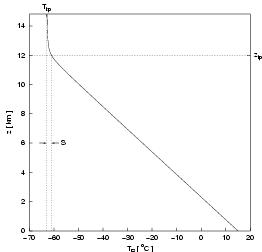
\includegraphics{Pics/Tr_z_Eng}
%\centering \epsfig{figure=Tr_z.Eng.eps, width=\linewidth}
\end{minipage}
\begin{minipage}{.5\linewidth}
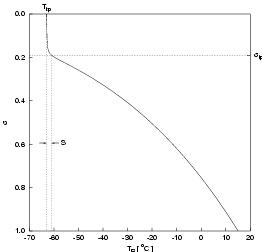
\includegraphics{Pics/Tr_sigma_Eng}
%\centering \epsfig{figure=Tr_sigma.Eng.eps, width=\linewidth}
\end{minipage}
\caption{\footnotesize{Vertical profile of the restoration temperature $T_R$ as 
function of the geometric height $z$ (left) and as function of the dimensionless 
vertical coordinate $\sigma$ (right) for standard parameter values: 
$(T_R)_{grd}=288\,K$; $z_{tp}=12\,km$; $L=6.5\,K/km$; $S=2\,K$.}} \label{Tr_z}
\end{figure}

The temperature contrast between low and high latitudes due to the differential 
radiative energy balance, which drives the general circulation, is described by 
the meridional form of the restoration temperature:
\begin{equation}
\label{Tr_phi}
T_R(\phi) = (\Delta T_R)_{NS}\, \frac{\sin\phi}{2}-(\Delta T_R)_{EP}\, \left(\sin^2\phi-\frac{1}{3}\right).
\end{equation}
The meridional gradient decreases with height and vanishes at the tropopause:
\begin{equation}
f(\sigma) = \left\{\ba{ll}
\di\sin\left(\frac{\pi}{2}\left(\frac{\sigma-\sigma_{tp}}{1-\sigma_{tp}}\right)\right) &
\mbox{if}\quad\sigma\ge\sigma_{tp} \\
0 &\mbox{if}\quad\sigma<\sigma_{tp},
\ea\right.
\end{equation}
with the height of the tropopause
\begin{equation}
\sigma_{tp} = \left(\frac{(T_R)_{tp}}{(T_R)_{grd}}\right)^{\frac{g}{LR}}.
\end{equation}
In equation (\ref{Tr_phi}), \dtepE represents the constant part of the meridional 
temperature contrast, and \dtns the variable part, corresponds to the annual cycle. 
Figure \ref{Tr_2d} shows the meridional and vertical form of the restoration 
temperature field (see eqn. (\ref{glgTr_2d})).

\afterpage{
\begin{figure}[!!!t]
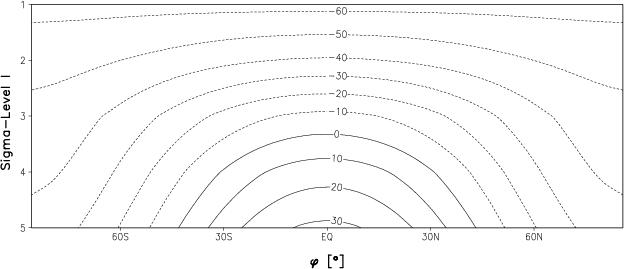
\includegraphics[width=16cm]{Pics/plot_Tr_aqua}
%\centering \epsfig{figure=plot_Tr_aqua.eps, angle=270, width=\linewidth}
\caption{\footnotesize{Restoration temperature field $T_R$ in $\degrees$C as function 
of latitude $\phi$ and the $\sigma$-level $l$ for standard parameter values as in 
figure \ref{Tr_z} and with $(\Delta T_R)_{EP}=70\,K$, $(\Delta T_R)_{NS}=0\,K$.}} \label{Tr_2d}
\end{figure}
}

Usually, for the lower model levels, the time scale $\tau_R$ is set to smaller values 
(stronger diabatic heating) than for the upper levels in order to account for the 
stronger impact of the turbulent heat fluxes near the surface. The standard $\tau_R$ setting 
for $n_l=5$ levels is $(\tau_R)_{l=1,\ldots,3}=30\,d$, $(\tau_R)_{l=4}=10\,d$, 
$(\tau_R)_{l=5}=5\,d$.

\subsection{Diffusion}
\label{diffusion}

The parameterizations (\ref{paraz}), (\ref{parad}) and (\ref{parat}) contain the 
hyperdiffusion terms $H_\zeta$, $H_D$ and $H_T$, respectively. The hyperdiffusion 
parameterizes both the subgrid scale horizontal mixing and the energy cascade into 
these scales and its subsequent dissipation, because the dissipative range of the 
wavenumber-energy-spectrum is not included with the relatively coarse model resolution. 
If $Q$ is one of the model variables $\zeta$, $D$ or $T$, then the hyperdiffusion 
is given by equation (\ref{hypergitter}) for grid point representation and by equation 
(\ref{hyperspektral}) for spectral representation (see also eqn. (\ref{spektral}))
\beqa
H & = & -(-1)^hK\,\nabla^{2h}\,Q(\lambda,\mu,t) \label{hypergitter} \\
  & = & -(-1)^hK\,\nabla^{2h}\sum_\gamma Q_\gamma(t)\,Y_\gamma(\lambda,\mu). \label{hyperspektral}
\eeqa
The hyperdiffusion for one spectral mode $\gamma$ is then \citep{holton}:
\beqa
H_\gamma & = & -(-1)^hK\,\nabla^{2h}\,Q_\gamma(t)\,Y_\gamma(\lambda,\mu) \\
         & = & -K\left(\frac{n(n+1)}{a^2}\right)^hQ_\gamma(t)\,Y_\gamma(\lambda,\mu). \label{hgamma.2}
\eeqa
With the condition that the spectral modes with $n=n_T$ are damped with a prescribed 
time scale $\tau_H$:
\begin{equation}
H_\gamma = -\frac{1}{\tau_H}\,Q_\gamma(t)\,Y_\gamma(\lambda,\mu)\quad\mbox{}
\end{equation}
${if} n=n_T,$ substitution into Equation (\ref{hgamma.2}) yields:
\begin{equation}
K = \frac{1}{\tau_H}\left(\frac{a^2}{n_T(n_T+1)}\right)^h.
\end{equation}
Thus, from Equation (\ref{hgamma.2}) it follows that:
\begin{equation}
H_\gamma = -\frac{1}{\tau_H}\left(\frac{n(n+1)}{n_T(n_T+1)}\right)^hQ_\gamma(t)\,Y_\gamma(\lambda,\mu). \label{hn2}
\end{equation}
In the model the hyperdiffusion is applied in the form (\ref{hn2}). For the shortest 
waves ($n=n_T$) the damping is maximal, for the mean ($n=0$) the damping vanishes. 
The integer exponent with the standard value $h=4$ leads to an additional reduction 
of the damping at small wavenumbers. The diffusion time scale is usually set to
 $\tau_H=1/4\,d$.
